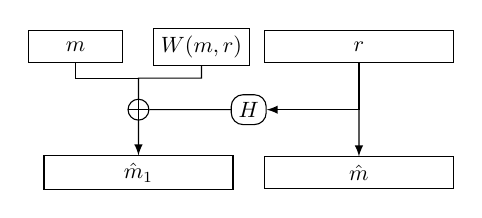
\begin{tikzpicture}[scale=0.8, every node/.style={scale=0.8}]
\node (m) [draw,minimum width=1.5cm, minimum height=0.5cm] {$m$};
\node (p0) at (2cm,0) [draw, minimum width=1.5cm, minimum height=0.5cm] {$W(m,r)$};
\node (r) at (4.5cm,0) [draw,minimum width=3cm, minimum height=0.5cm] {$r$};

\node (xor) at (1cm,-1cm) [circle, draw] {};
\draw[-] (xor.north) -- (xor.south);
\draw[-] (xor.east) -- (xor.west);
%\node (xor2) at (4.5cm,-2cm) [circle, draw] {};
%\draw[-] (xor2.north) -- (xor2.south);
%\draw[-] (xor2.east) -- (xor2.west);

\node (G) at (2.75cm,-1cm) [draw,rounded corners=1ex] {$H$};
%\node (H) at (2.75cm,-2cm) [draw,rounded corners=1ex] {$H$};

\node (m1) at (1cm,-2cm) [draw,minimum width=3cm, minimum height=0.5cm] {$\hat{m}_1$};
\node (mh) at (4.5cm,-2cm) [draw,minimum width=3cm, minimum height=0.5cm] {$\hat{m}$};

\draw [-] (m) |- (1cm,-0.5cm);
\draw [-] (p0) |- (1cm,-0.5cm) -- (xor);
\draw [-] (xor) -- (G);
\draw [-latex] (r) |- (G);
%\draw [-latex] (xor) |- (H);
%\draw [-] (r) |- (H);
\draw [-latex] (xor) -- (m1);
\draw [-latex] (r) -- (mh);
\end{tikzpicture}